\section{5-state Sporadic Machines}\label{sec:sporadic}



\begin{figure}[h!]
    \centering

    % First row: 3 images
    \begin{minipage}{\textwidth}
        \centering
        \begin{subfigure}{0.3\textwidth}
            \centering
            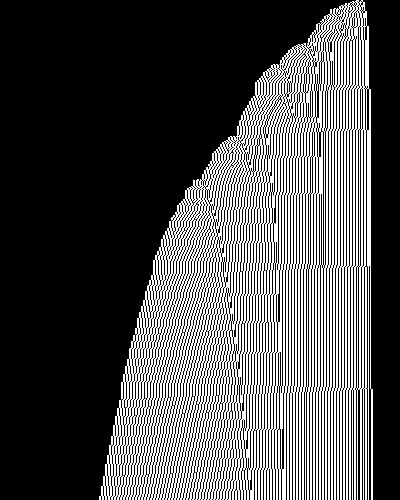
\includegraphics[width=\linewidth]{figures/sporadic-machines/sk1.png}
            \caption*{\href{https://bbchallenge.org/1RB1RD_1LC0RC_1RA1LD_0RE0LB_---1RC}{Skelet \#1}}
        \end{subfigure}
        \hfill
        \begin{subfigure}{0.3\textwidth}
            \centering
            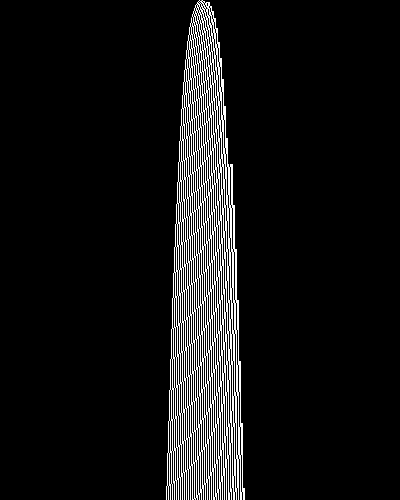
\includegraphics[width=\linewidth]{figures/sporadic-machines/sk17.png}
            \caption*{\href{https://bbchallenge.org/1RB---_0LC1RE_0LD1LC_1RA1LB_0RB0RA}{Skelet \#17}}
        \end{subfigure}
        \hfill
        \begin{subfigure}{0.3\textwidth}
            \centering
            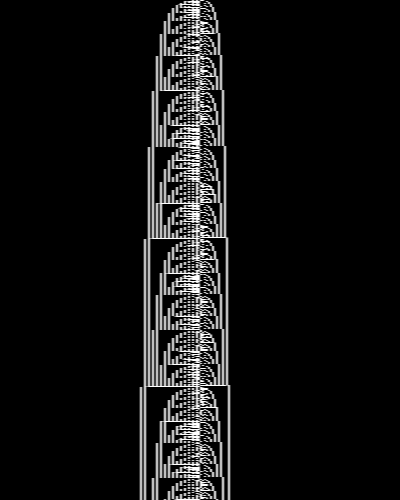
\includegraphics[width=\linewidth]{figures/sporadic-machines/sk10.png}
            \caption*{\href{https://bbchallenge.org/1RB0RA_0LC1RA_1RE1LD_1LC0LD_---0RB}{Skelet \#10}}
        \end{subfigure}
    \end{minipage}

    \vspace{1.5em}

    % Second row: Shift Overflow Counters
    \begin{tikzpicture}
        \node[draw=magenta, thick, rounded corners, inner sep=8pt] (box1) {
            \begin{minipage}{0.95\textwidth}
                \centering
                \textbf{\textcolor{magenta}{Shift Overflow Counters}}\\[0.8em]
                \begin{subfigure}{0.17\textwidth}
                    \centering
                    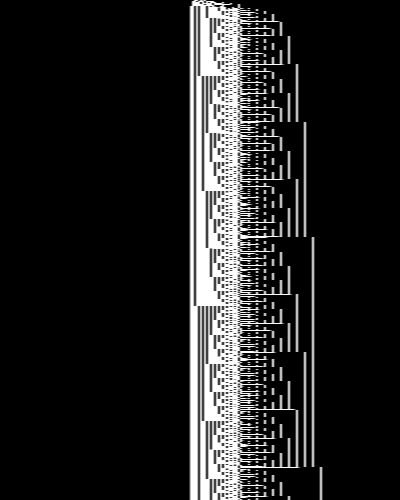
\includegraphics[width=\linewidth]{figures/sporadic-machines/soc_sk15.png}
                    \caption*{\href{https://bbchallenge.org/1RB---_1RC1LB_1LD1RE_1LB0LD_1RA0RC}{Skelet \#15}}
                \end{subfigure}
                \hfill
                \begin{subfigure}{0.17\textwidth}
                    \centering
                    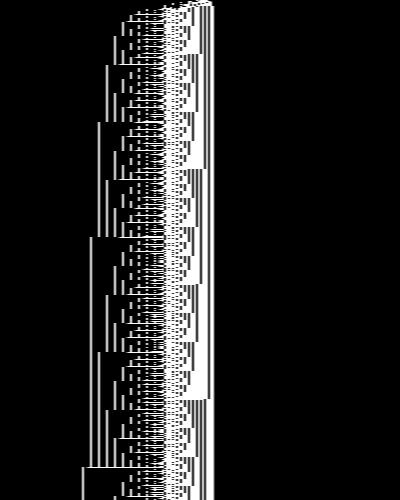
\includegraphics[width=\linewidth]{figures/sporadic-machines/soc_sk26.png}
                    \caption*{\href{https://bbchallenge.org/1RB1LD_1RC0RB_1LA1RC_1LE0LA_1LC---}{Skelet \#26}}
                \end{subfigure}
                \hfill
                \begin{subfigure}{0.17\textwidth}
                    \centering
                    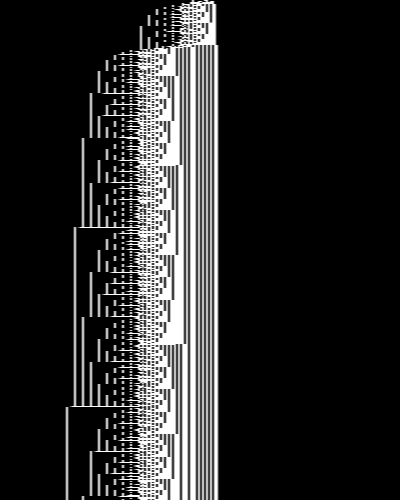
\includegraphics[width=\linewidth]{figures/sporadic-machines/soc_sk33.png}
                    \caption*{\href{https://bbchallenge.org/1RB1LC_0RC0RB_1LD0LA_1LE---_1LA1RE}{Skelet \#33}}
                \end{subfigure}
                \hfill
                \begin{subfigure}{0.17\textwidth}
                    \centering
                    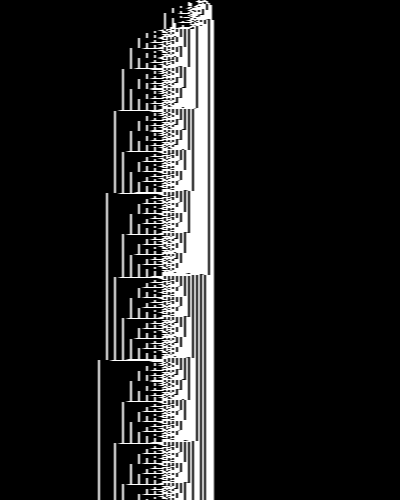
\includegraphics[width=\linewidth]{figures/sporadic-machines/soc_sk34.png}
                    \caption*{\href{https://bbchallenge.org/1RB1LC_0RC0RB_1LD0LA_1LE---_1LA1RA}{Skelet \#34}}
                \end{subfigure}
                \hfill
                \begin{subfigure}{0.17\textwidth}
                    \centering
                    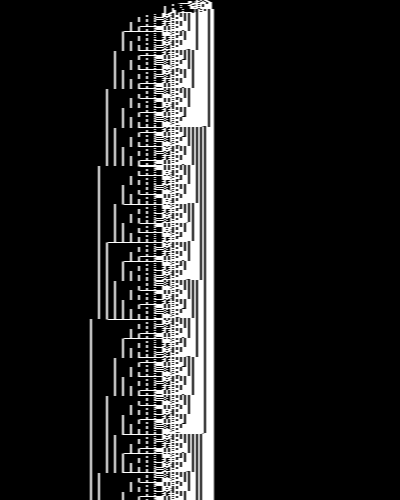
\includegraphics[width=\linewidth]{figures/sporadic-machines/soc_sk35.png}
                    \caption*{\href{https://bbchallenge.org/1RB1LC_0RC0RB_1LD0LA_1LE---_1LA0LA}{Skelet \#35}}
                \end{subfigure}
            \end{minipage}
        };
    \end{tikzpicture}

    \vspace{1.5em}

    % Third row: Finned Machines
    \begin{tikzpicture}
        \node[draw=magenta, thick, rounded corners, inner sep=8pt] (box2) {
            \begin{minipage}{0.95\textwidth}
                \centering
                \textbf{\textcolor{magenta}{Finned Machines}}\\[0.8em]
                \begin{subfigure}{0.17\textwidth}
                    \centering
                    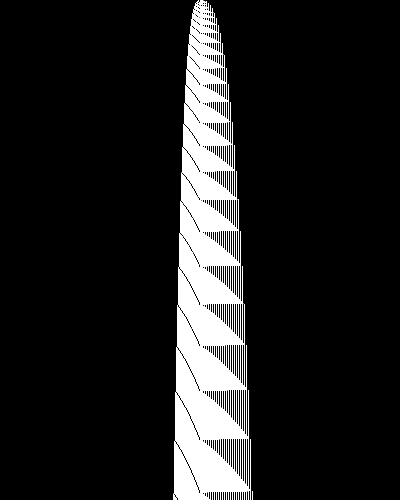
\includegraphics[width=\linewidth]{figures/sporadic-machines/finned_1.png}
                    \caption*{\href{https://bbchallenge.org/1RB0LE_1RC1RB_1RD1LC_0LE0RB_---1LA}{Finned \#1}}
                \end{subfigure}
                \hfill
                \begin{subfigure}{0.17\textwidth}
                    \centering
                    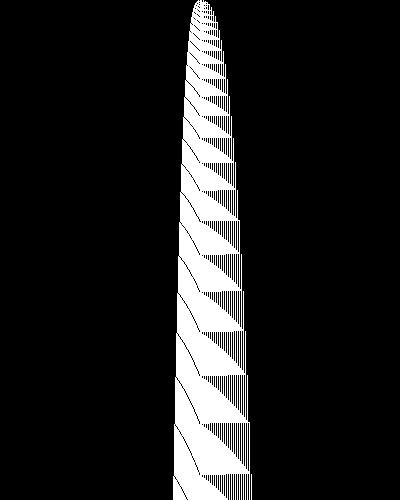
\includegraphics[width=\linewidth]{figures/sporadic-machines/finned_2.png}
                    \caption*{\href{https://bbchallenge.org/1RB1RA_1RC1LB_0LD0RA_1RA1LE_---0LD}{Finned \#2}}
                \end{subfigure}
                \hfill
                \begin{subfigure}{0.17\textwidth}
                    \centering
                    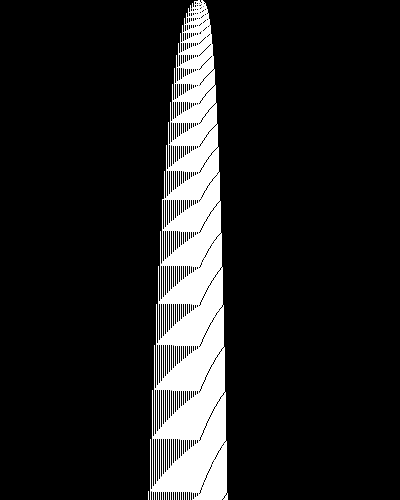
\includegraphics[width=\linewidth]{figures/sporadic-machines/finned_3.png}
                    \caption*{\href{https://bbchallenge.org/1RB1RE_1LC1RB_0RA0LD_1LB1LD_---0RA}{Finned \#3}}
                \end{subfigure}
                \hfill
                \begin{subfigure}{0.17\textwidth}
                    \centering
                    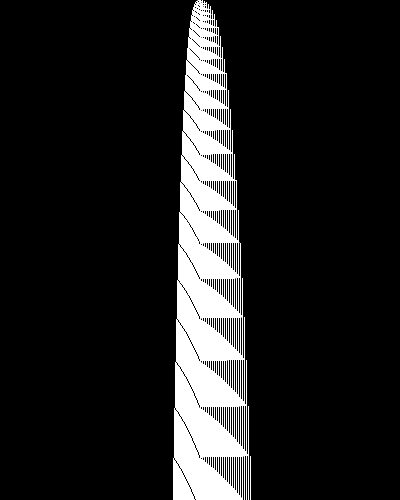
\includegraphics[width=\linewidth]{figures/sporadic-machines/finned_4.png}
                    \caption*{\href{https://bbchallenge.org/1RB1LA_0LC0RE_---1LD_1RA0LC_1RA1RE}{Finned \#4}}
                \end{subfigure}
                \hfill
                \begin{subfigure}{0.17\textwidth}
                    \centering
                    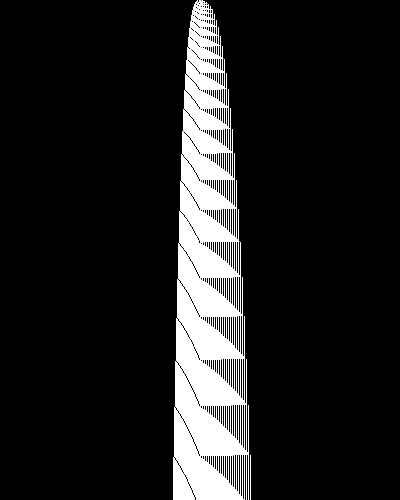
\includegraphics[width=\linewidth]{figures/sporadic-machines/finned_5.png}
                    \caption*{\href{https://bbchallenge.org/1RB1LA_0LC0RE_---1LD_1LA0LC_1RA1RE}{Finned \#5}}
                \end{subfigure}
            \end{minipage}
        };
    \end{tikzpicture}

    \caption{Family picture of the 5-state Sporadic Machines (20,000-step space-time diagrams) which required individual \Coq nonhalting proofs; machine names in the Figure are clickable URLs giving the TNF-normalised transition table of each machine (see Section~\ref{sec:enum}). All Sporadic Machines were also identified by Skelet \cite{Skelet_bbfind}, either as unprovable using his \texttt{bbfind} program, or, for what we call ``Finned machines'' marked as ``easily provable by hand'' \cite{Skelet_bbfind_list}. For better visibility, diagrams of counters (Skelet \#10 and Shift Overflow Counters) have been represented using a tape of length 200 instead of 400, giving a \textit{zoomed-in} effect.}
    \label{fig:machine_overview}
\end{figure}

